\documentclass{article}

\usepackage[paperheight=11in,paperwidth=8.5in,top=1.5in,bottom=1.5in,right=1in,left=1in]{geometry}

\usepackage{url}
\usepackage[latin1]{inputenc}
\usepackage{graphicx}
\usepackage{pdflscape}
\usepackage{algorithmic}

%%%%%%%%%%%%%%%%%%%%%%%%%%%%%%%%%%%%%%%%%%%%%%%%%%%%%%%%%%%%%%%%%%%%%%%%%%%%%%
% front page
%%%%%%%%%%%%%%%%%%%%%%%%%%%%%%%%%%%%%%%%%%%%%%%%%%%%%%%%%%%%%%%%%%%%%%%%%%%%%%

\begin{document}

%\begin{frontmatter}


\title{High performance evolutionary algorithms on GPUs: a survey}

\author{P. Garc{\'\i}a-S{\'a}nchez$^1$, A.M. Mora$^2$,Gustavo Romero$^3$\\
  J. J. Merelo$^1$, P.A. Castillo$^3$, Antonio Fern�ndez-Ares$^2$  \\ \\
\small{$^1$ Dept. Computer Engineering, University of C{\'a}diz (Spain)}\\
\small{$^2$ Dept. Signal Theory, Telematics and Communications,}\\
\small{ETSIIT-CITIC, University of Granada (Spain)}\\
\small{$^3$ Dept. Computer Architecture and Computer Technology,}\\
\small{ETSIIT-CITIC, University of Granada (Spain)}\\
\small{\texttt{pablo.garciasanchez@uca.es}}\\
\small{\texttt{\{amorag,gustavo,jmerelo,pacv,mgarenas,antares\}@ugr.es}}
}

\maketitle

\begin{abstract}
Evolutionary Algorithms (EAs), a population based stochastic approach to problem solving, have been widely adapted to be run on Graphics Processing Units (GPUs), using the fact that the different solutions in the population can be evaluated in parallel. Beyond that fact, different methodologies and techniques are used; this paper aims first to describe the parallelization process of EAs on GPUs, introducing their general features and main distributed models, together with several frameworks which allow to conduct this task easily in a review of the new advances in hardware and software in this field, as well as new trends and challenges arising in this scope; and, second the main issues to take into account in order to carry out these parallel implementations.
Thus, a selected sample of the publications have been reviewed, extracting their key features to categorize them. 
The papers have been grouped following a taxonomy of the approaches used for GPGPU parallelization. 
Then, a more in-depth review has been conducted on the most
representative works in each category, extracting their main features
and findings, and some statistical analyses on the publication history
and tendency have been conducted. After this review, a summary of research challenges and future trends of research are presented, to provide insights about how this field can still be addressed.
% Antonio - Rewrite this with the final contents of the paper, as they are changing
\end{abstract}

{\bf Keywords:}: Parallel computation,  evolutionary algorithms,
metaheuristics, GPUs, GPGPU computing, survey.


%%%%%%%%%%%%%%%%%%%%%%%%%%%%%%%%%%%%%%%%%%%%%%%%%%%%%%%%%%%%%%%%%%%%%%%%%%%%%%
\section{Introduction}
\label{sec:intro}
%%%%%%%%%%%%%%%%%%%%%%%%%%%%%%%%%%%%%%%%%%%%%%%%%%%%%%%%%%%%%%%%%%%%%%%%%%%%%%

GPUs (Graphics Processing Unit) are processors that are optimized for
dealing with data streams, and in order to perform that task they are
composed of hundreds (or thousands) of computation units designed
to perform graphics manipulations applying optimized graphical
primitive operations, at a higher throughput than general purpose
CPUs. However, high performance in processing vectors is not only
needed in the realm of games and image rendering, which is why they
have been adapted to be used either as general purpose
multi-processors with shared memory, or as Single Instruction
Multiple Data (SIMD) processors \cite{Pharr12SPMD}; their utilization
as general purpose processors is usually called GPGPU programming
\cite{luebke2006gpgpu,owens2007}.  
Their use in all kind of computers inspired the development of 
specific programming languages, tools and applications that leverage
the power of their architecture, favouring the emergence of specific
solutions, frameworks and algorithms that take advantage of them.

Our paper in 2012 \cite{arenas2012gpu} reviewed the state of the art
back then; since that paper was published, new ways of using GPUs for
solving any kind of problem have been introduced, from cloud instances that include them to
{\em desktop supercomputers} that boast several GPU linked by a
high-performance network. These advances have extended the use of
GPGPU programming and algorithms to many other labs and
even, given that every computer nowadays has a powerful graphics card,
to almost every one, extending the range of applications from speeding
up desktop programs to very high performance data processing.


This also means that the field that is the focus of this paper,
Evolutionary Algorithms (EAS) \cite{de2016evolutionary}, has been one
of the general problems to which GPUs have been applied. EAs are a biologically
inspired class of algorithms that, in general, {\em evolve} a set of
solutions (usually called a {\em population}) by assigning a score
(called {\em fitness}) to every solution and selecting them for
reproduction so that those with the higher fitness get more copies in
the reproductive pool. That pool is then changed blindly (in a
procedure called {\em mutation}),  and combined (in a procedure
usually called {\em crossover}) to create a new population on which
the process is repeated until the solution, or a suitable one is found. 


This metaheuristic has been widely used in the literature to solve
many different problems, due to its simplicity and straightforward
implementation. However, the application of EAs to find the solution
of either real world problems or large instances of some benchmark
problems, requires a high amount of computational power. Thus, it is
quite frequent to design a parallel or distributed version of this
kind of algorithms. 

Even if the most common form of an EA is sequential, the fact that they operate on populations of solutions, with operators applied to a single individual at a time, make them amenable to a straightforward, and functionally equivalent,
parallel version, and thus, very suitable to be distributed at different grain levels. 
The aim of the parallelization is usually the improvement of the
running time for yielding an objective solution, if known, or for
obtaining a certain degree of quality in the solution, if it is not
the optimal. But sometimes this distribution also implies a different
searching scheme, which leads to a different searching area of the
space of solutions which would change the number of evaluations needed
to find the solution. For these reasons, parallel EAs have been widely studied in the literature, so this survey will be focused on how to implement them
using general purpose computing on GPU techniques. 


This paper presents a taxonomy regarding the different
parallelization models, along with a complete survey of the most
relevant proposals in this scope, extracted after reviewing more than
200 works published since their emergence in 2004.
% Antonio - Update these numbers

In addition, the manuscript describes the main concepts related with
GPUs, from their internal architecture, to the usual programming
models and structures, through several widely used tools and
frameworks which can help to do this task. After this introduction, the work gives some guidelines to parallelize an EA using GPUs, pointing out their suitability as well as the main issues and constraints that should be taken into account.

%The work also compares this parallelization methodology with other extended high-performance methods such as Cloud Computing, massive Volunteer Computing, or specialized FPGAs.
% Antonio - This has been removed.

Finally, some of the new trends and open challenges in the scope of
GPGPU computing are discussed.

The rest of the paper is structured as follows: Section \ref{sec:eas}
introduces EAs and describes the most usual parallelization and
distribution models in the literature.  In Section
\ref{sec:parall_and_GPUs}, the internal structure of GPUs and their
utility for GPGPU computing are described, as well as a comparison of the
existing cards in the market is shown.  Then, programming schemes,
languages and tools used in GPUs are presented in Section
\ref{sec:programming}, followed by a description of the best
frameworks used to parallelize EAs in order to take advantage of the
power of GPUs (Section \ref{sec:parallelizing}). In the same
section, the main issues to consider when a parallel version of an EA
wants to be implemented on a GPU, are commented.  Next, Section
\ref{sec:taxonomy} proposes a taxonomy based on the different parallel
models implemented in the literature, in order to categorize the
reviewed papers. Thus, in Section \ref{sec:survey} a set of
representative works (according to their number of citations)
describing different approaches using GPUs are reviewed and divided
following the proposed taxonomy, plotting also some interesting
numbers and graphs related to them.  New trends and challenges are discussed in Section \ref{sec:discussion}. Finally, Section \ref{sec:conclusions} remarks
reached conclusions.
% Antonio - Revise and rewrite this structure once the paper is finished, as now we are removing and merging sections.

%%%%%%%%%%%%%%%%%%%%%%%%%%%%%%%%%%%%%%%%%%%%%%%%%%%%%%%%%%%%%%%%%%%%%%%%%%%%%%%
\section{Evolutionary Algorithms}
\label{sec:eas}
%%%%%%%%%%%%%%%%%%%%%%%%%%%%%%%%%%%%%%%%%%%%%%%%%%%%%%%%%%%%%%%%%%%%%%%%%%%%%%%

This section gives a general overview of the most used types of
Evolutionary Algorithms (EAs) describing their common elements. In
addition, the most extended models to parallelize EAs are presented,
to understand all their possible architectural possibilities. 

EAs are a set of bioinspired techniques applied to optimization problems \cite{eiben2010whatis}, based on the process of natural selection \cite{darwin1859}. In this kind of pseudo-stochastic algorithms, a \textit{population} of codified solutions (called \textit{individuals}) is created. There is also a \textit{fitness} function, which evaluates the level of adaptation of the individuals to the problem to solve.
Thus, the fittest individuals have more chances to be selected for
reproduction, so their offspring could inherit their genetic
material. Due to the nature of GPGPU computing, two types of
evolutionary algorithms are specially suitable for them: globally
parallel and spatially structured EAs.

Global parallel evolutionary algorithms are also called called the \textit{Farming model},
\textit{client-server} or \textit{Centralized EAs}; in them the parallelism is
applied is only applied at the evaluation level, with a central node or server coordinating several
client nodes, which in this context would be GPU computing nodes. The
central node runs a sequential EA, but it
distributes the individuals of the population among the clients just
for being evaluated. Figure \ref{fig:serverClient} depicts this
approach.
%
\begin{figure}[tb]
\centering
%\includegraphics[width=20pc]{gfx/distributed/serverClient.jpg}
\includegraphics[width=20pc]{serverClient}
\caption{Client-server model.}
\label{fig:serverClient}
\end{figure}

Spatially structured algorithms, however, are parallel at the
population level, that is, the population is divided and distributed
among the different computing elements. Depending on how the
distribution is performed they are qualified with different {\em
  grains} or amount of computation performed at a local level. 

\begin{description}
\item[Coarse-grained] In which independent subsets of individuals are considered. One of the most extended approaches is the \textit{Island model}, where a number of nodes execute simultaneously the EA, working with different sub-populations at the same time. Each certain number of generations some individuals are interchanged (migrated) between populations. Figure \ref{fig:ring} shows this model with a ring topology.
%
\begin{figure}[tb]
\centering
%\includegraphics[width=20pc]{gfx/distributed/ring.jpg}
\includegraphics[width=20pc]{ring}
\caption{Island model scheme using a neighbourhood ring topology.}
\label{fig:ring}
\end{figure}

\item[Fine-grained approach] In this approach, also called \textit{Cellular EA} (CEA) \cite{alba-cellular-2008}, each node has one individual of the population, and selection and reproduction are limited to the individuals on the neighbourhood of every node. Usually a bi-dimensional grid is used as topology, such as the one shown in Figure \ref{fig:cellular}.
%
\begin{figure}[tb]
\centering
%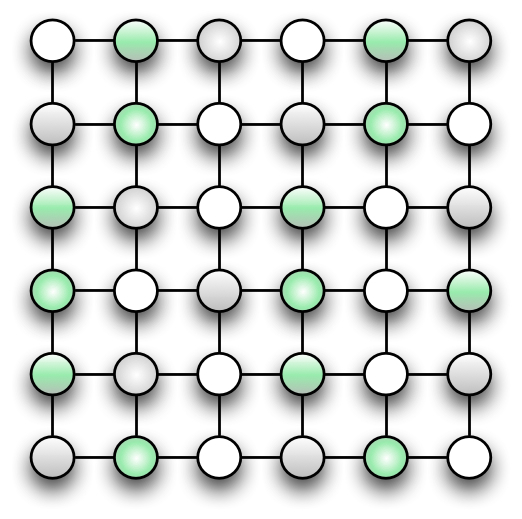
\includegraphics[width=5cm]{gfx/distributed/cellular.jpg}
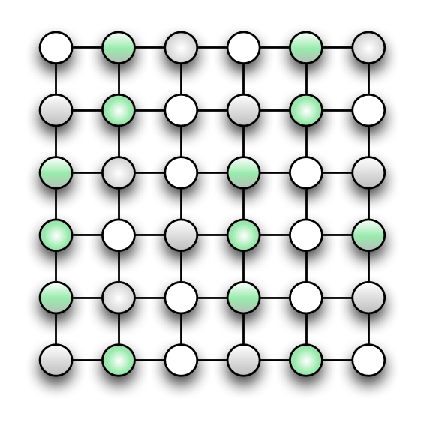
\includegraphics[width=15pc]{cellular}
\caption{Cellular Evolutionary Algorithm.}
\label{fig:cellular}
\end{figure}

\end{description}

%%%%%%%%%%%%%%%%%%%%%%%%%%%%%%%%%%%%%%%%%%%%%%%%%%%%%%%%%%%%%%%%%%%%%%%%%%%%%%%
\section{GPU Programming and metaheuristics}
\label{sec:programming}
%%%%%%%%%%%%%%%%%%%%%%%%%%%%%%%%%%%%%%%%%%%%%%%%%%%%%%%%%%%%%%%%%%%%%%%%%%%%%%%

This section introduces the most relevant concepts to know before
using GPUs for General Purpose computing (GPGPU computing). These aspects normally
differ between vendors, but they have common features which we 
describe here: the different programming possibilities, the execution
model that GPU computing follows, and the memory scheme to use,
concluding on how this affects the implementation of diverse metaheuristic
algorithms.

Parallel computation has passed from been an enhancement to regular computing to a necessity due to the space and miniaturization limitations predicted by Moore's and Koomey's Laws \cite{10.1109/MAHC.2010.28}. 
As newer processors are just marginally faster than previous ones
the only way to take advantage of the amount of transistors is putting
many cores together. For many years, clock rates and instruction-level
parallelism has become fast enough to allow faster execution of the
same payload on a new processor without modification. Adding heat to
this equation has finally forced chip makers to favor multi-core
designs. Now the only way to benefit from many cores is multi-threaded
software \cite{6307773} and languages
\cite{DBLP:conf/evoW/GuervosLCVG19}. 

At the same time graphic cards became general-purpose devices long
time ago. Indeed, earliest academic work about general purpose
computing on GPUs date back to 2002 at the University of Washington
\cite{Thompson:2002:UMG:774861.774894}, and 2004 in Stanford
\cite{Buck:2004:BGS:1015706.1015800}; in fact, before multicore
processors became a commodity, GPUs included in every computer were
able to use their many cores.
GPUs have
been integrated inside CPUs from 2006 in budget desktop PCs
as well as in mobile phones for many years. Over time the use of the GPUs
has grown a lot as they became cheaper. Many heavy tasks
have been parallelized like, for example, web page
rendering. %reference - JJ
This speed up is not trouble free because in order to be able to completely profit from GPUs our applications must be rewritten in a parallel fashion. 
% Not really - JJ
% Antonio - I have added a key word to make this sentence true. We cannot say in this paper that it is not needed to parallelize.

GPUs and CPUs are similar in many ways but there is one key
difference: the philosophy of how to execute a workload. The main
design purpose of a CPU core is the fast execution of a single thread of
code. GPUs, on the other side, pursue to maximize the throughput of
multithreaded streams of instructions and data. Another difference is the scheduling of threads: For
CPUs, the operating system schedule threads over free cores in a
competitive way. GPUs does it cooperatively with the help from
dedicated hardware. Some of this characteristics are shown in 
Figure \ref{fig:cpu-gpu}.

\begin{figure*}[!ht]
\centering
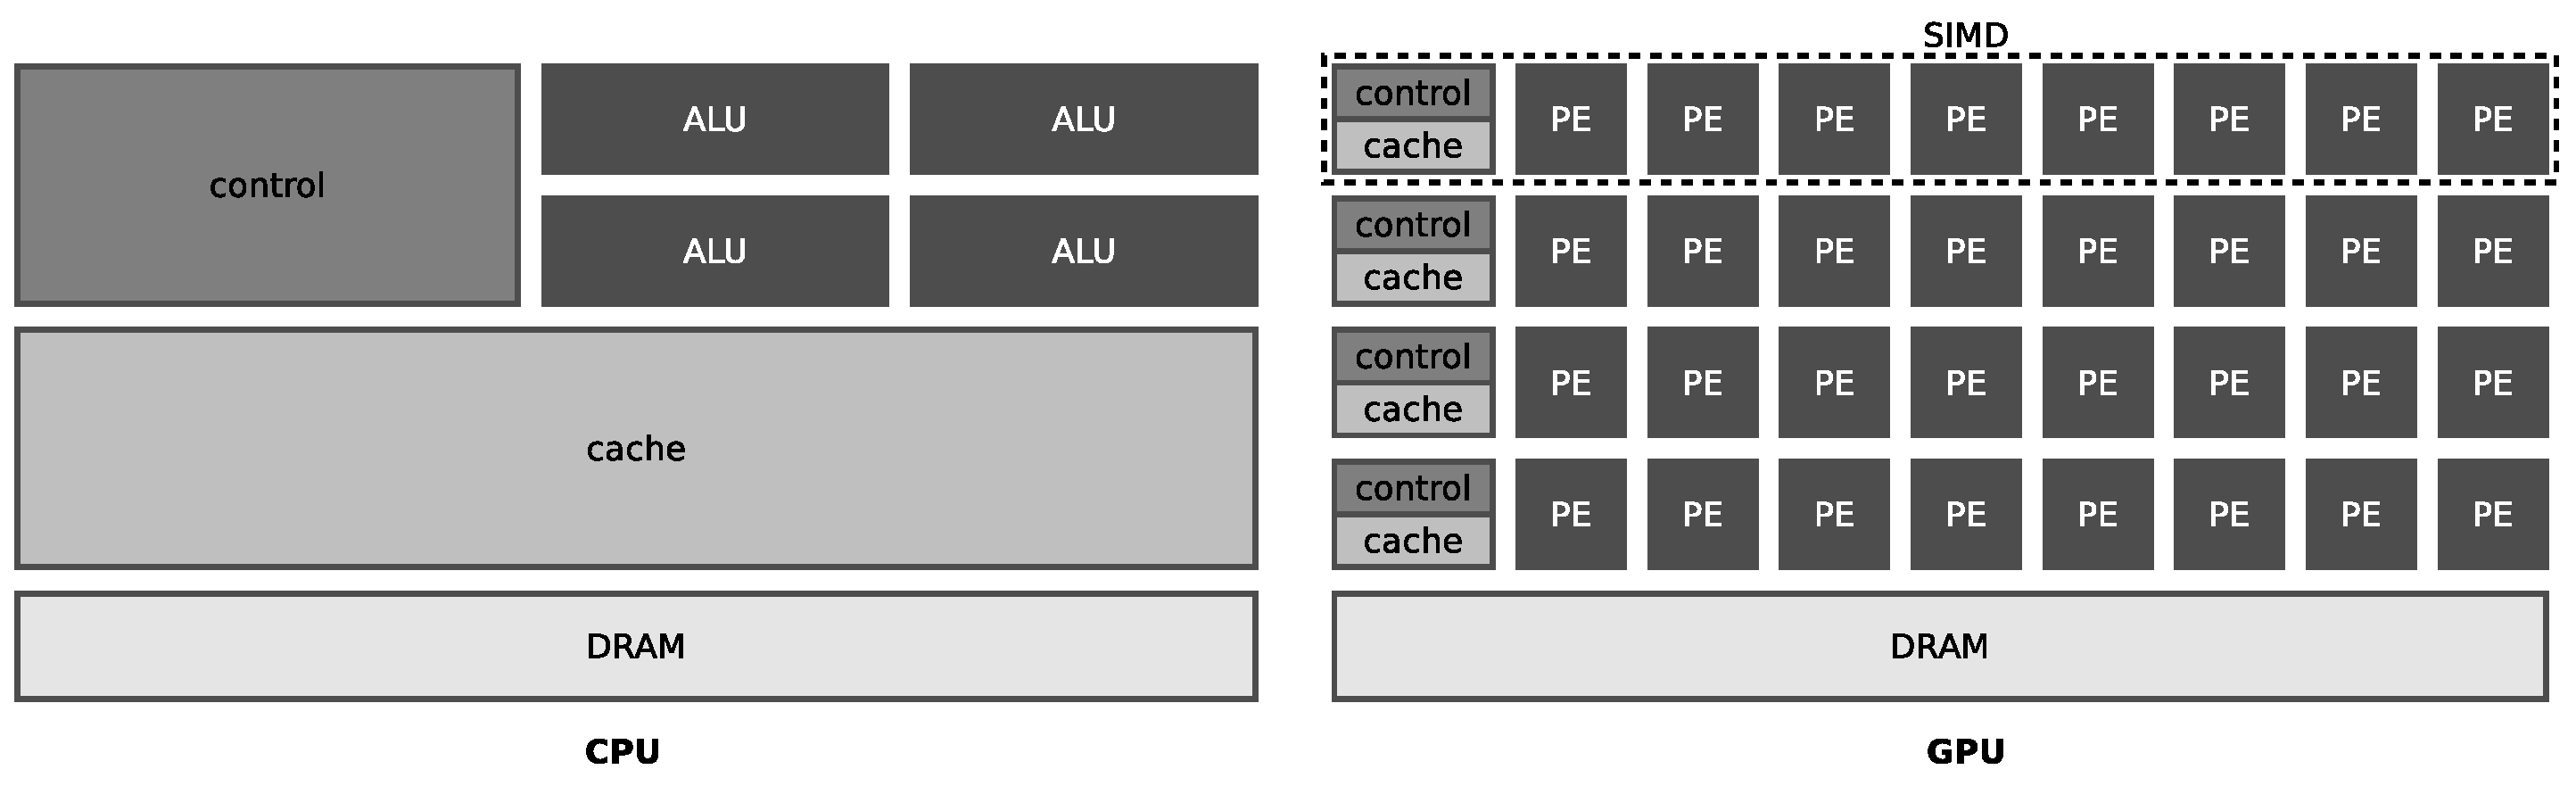
\includegraphics[width=\textwidth]{cpu-gpu}
\caption{CPU and GPU block diagram comparison. PE is a processing
  element, ALU stands for Arithmetic Logic Unit. DRAM is the dynamic RAM.}
\label{fig:cpu-gpu}
\end{figure*}

The trend observed with CPUs of integrating many companion cores
inside is now becoming true with the GPU also. The main reason is the
lower cost of the complete system. They only remain separate in
powerful systems with top processors and a low-demanding graphic content.
% What is that? - JJ
% Antonio - I guess it is clearer now


%%%%%%%%%%%%%%%%%%%%%%%%%%%%%%%%%%%%%%%%%%%%%%%%%%%%%%%%%%%%%%%%%%%%%%%%%%%%%%%
\subsection{Programming Model}
%%%%%%%%%%%%%%%%%%%%%%%%%%%%%%%%%%%%%%%%%%%%%%%%%%%%%%%%%%%%%%%%%%%%%%%%%%%%%%%

At the beginning, to benefit from GPU computational power, we had to learn about its internal design. The closer to the bare metal, the better. With the pass of time several Application Program Interfaces (APIs) have appeared to alleviate this inconvenience. The problem, again, is that every manufacturer designed its own proprietary one: AMD created Close to Metal and nVidia created CUDA. Over time a truly open and universal standard was introduced, OpenCL \cite{opencl}. It works even on Intel hardware. Today it is supported by all vendors. Only nVidia keeps pushing its own, CUDA, at the same time. OpenCL was initially developed by Apple who pass it to Khronos Group for open and free release. At the same time Microsoft created DirectX for its operating systems.

OpenCL aspired to reach fame in the same way that OpenGL. The first with heterogeneous computing and the second in the graphics world. OpenCL is cross-platform and very inclusive about software and hardware. Primarily targeting GPUs but also capable of running on multi-core CPUs and FPGAs. Applications can be made portable across operating systems and hardware platforms keeping functionality and correctness. The first implementation was release in 2009.

Most APIs are based on C-like languages but with some constraints in order to improve its parallel throughput. Usual limitations are avoiding recursion and restricting pointer usage to a minimum. Apart from GNU GCC, another open source compiler is gaining relevance, LLVM \cite{LLVM} from the University of Illinois.

Developers are now working hard to delight new user with libraries that make using the GPU very easy. Some examples of this are the C++ parallel extensions of STL and the incorporation of GPU offloading in OpenMP into GCC version 7. A very interesting comparison of many modern C++ parallel libraries on top of CUDA and OpenCL can be found in \cite{doi:10.1137/120903683}.

%%%%%%%%%%%%%%%%%%%%%%%%%%%%%%%%%%%%%%%%%%%%%%%%%%%%%%%%%%%%%%%%%%%%%%%%%%%%%%%
\subsection{Execution Model}
%%%%%%%%%%%%%%%%%%%%%%%%%%%%%%%%%%%%%%%%%%%%%%%%%%%%%%%%%%%%%%%%%%%%%%%%%%%%%%%

Most APIs mentioned are designed with heterogeneous computing in
mind. They use a traditional CPU and an optional GPU in the case that
one, or more, are present. In every parallel application we can find
mixture of serial and parallel parts. This way, serial parts are
executed on the CPU and parallel parts, designated \textit{kernels},
may execute on any parallel device, the CPU or the GPU, as long as
synchronization is enforced between both parts. OpenCL is aimed at
task and parallel data while CUDA and DirectCompute, a part of
DirectX, only target are data parallelism.

A kernel executes a single set of instructions over an usually large
quantity of data. Data is organized in the shape of 1 to 3
multidimensional arrays. In the OpenCL terminology, a
\textit{work-item} is a
piece of data in the sense previously described. One kernel is
responsible for the execution of many work-items but it use to divide
then in more manageable \textit{work-groups} of smaller size. These
way a kernel may execute 32K work-items, composed of 64 work-groups of
512 items each.

One of the strongest limitations compared to general computing is the
communication between kernels. Communication and synchronization
within work-groups works as we are used but not further. In this
sense, a work-group serves two purposes: breaking a kernel in more
manageable, and easily shareable, chunks and defining a limit to fast, or
possible, communications.

\begin{figure*}[!ht]
\centering
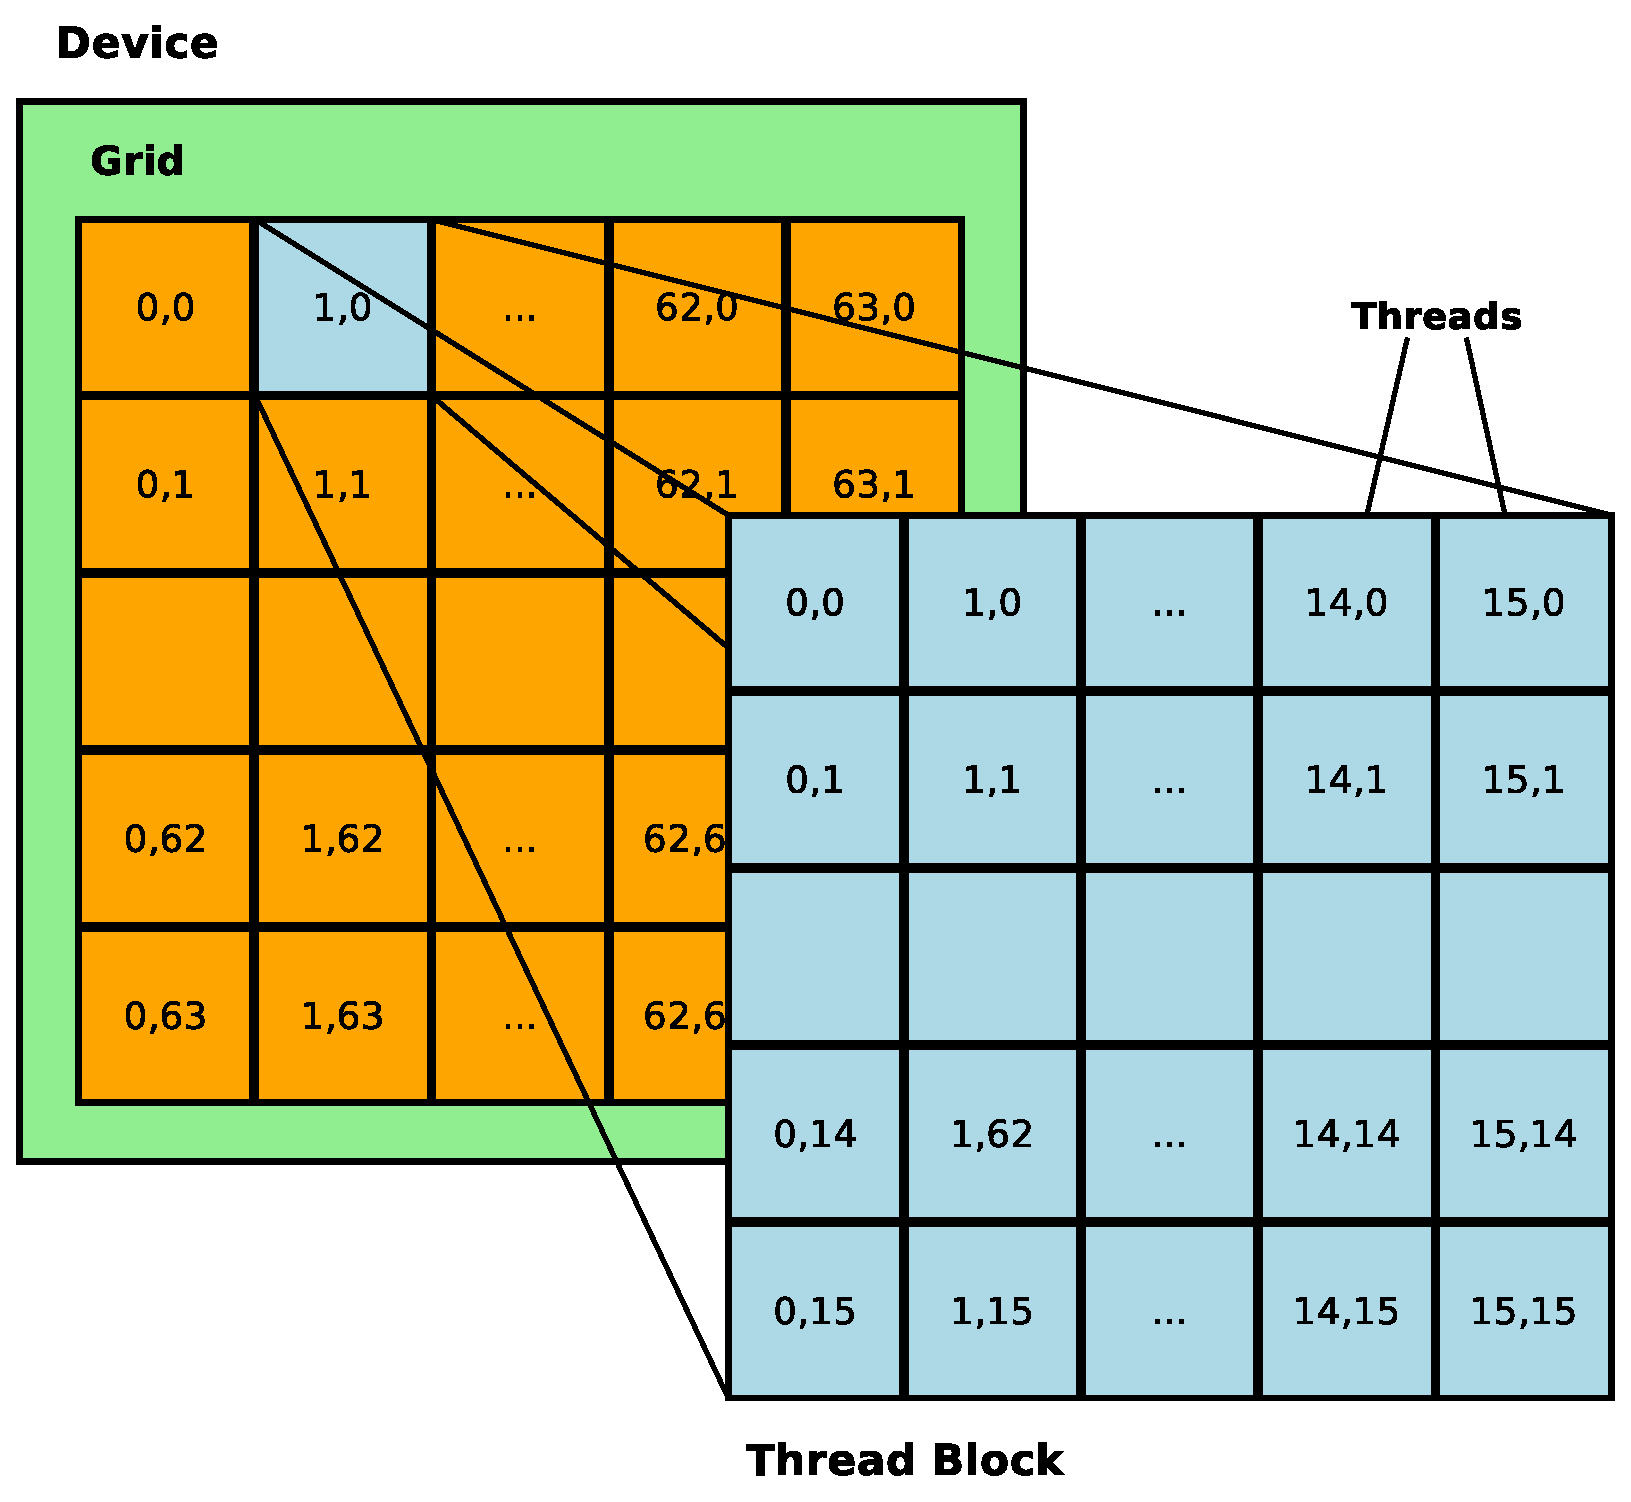
\includegraphics[width=0.9\textwidth]{grid}
\caption{Execution model: A piece of data is called {\it work-item} (thread); a kernel has many work-items subdivided into many {\it work-groups} (thread blocks); each work-group process many work-items.}
\label{figure:grid}
\end{figure*}


%%%%%%%%%%%%%%%%%%%%%%%%%%%%%%%%%%%%%%%%%%%%%%%%%%%%%%%%%%%%%%%%%%%%%%%%%%%%%%%
\subsection{Memory Model}
%%%%%%%%%%%%%%%%%%%%%%%%%%%%%%%%%%%%%%%%%%%%%%%%%%%%%%%%%%%%%%%%%%%%%%%%%%%%%%%

Programmers in general are used to read and write freely in any type of memory. Using the CPU we can read and write from registers, local memory (stack), global memory (heap) and disk. Accessing data for a GPU is more restricted.

Data storage and communication within a device and between devices, mainly CPU and GPU, is dictated by the memory model. It can represented in Figure \ref{figure:memory}. Again, every vendor use the same four memory types but with a different name. This is true for DirectCompute, CUDA and OpenCL.

\begin{figure*}[!ht]
\centering
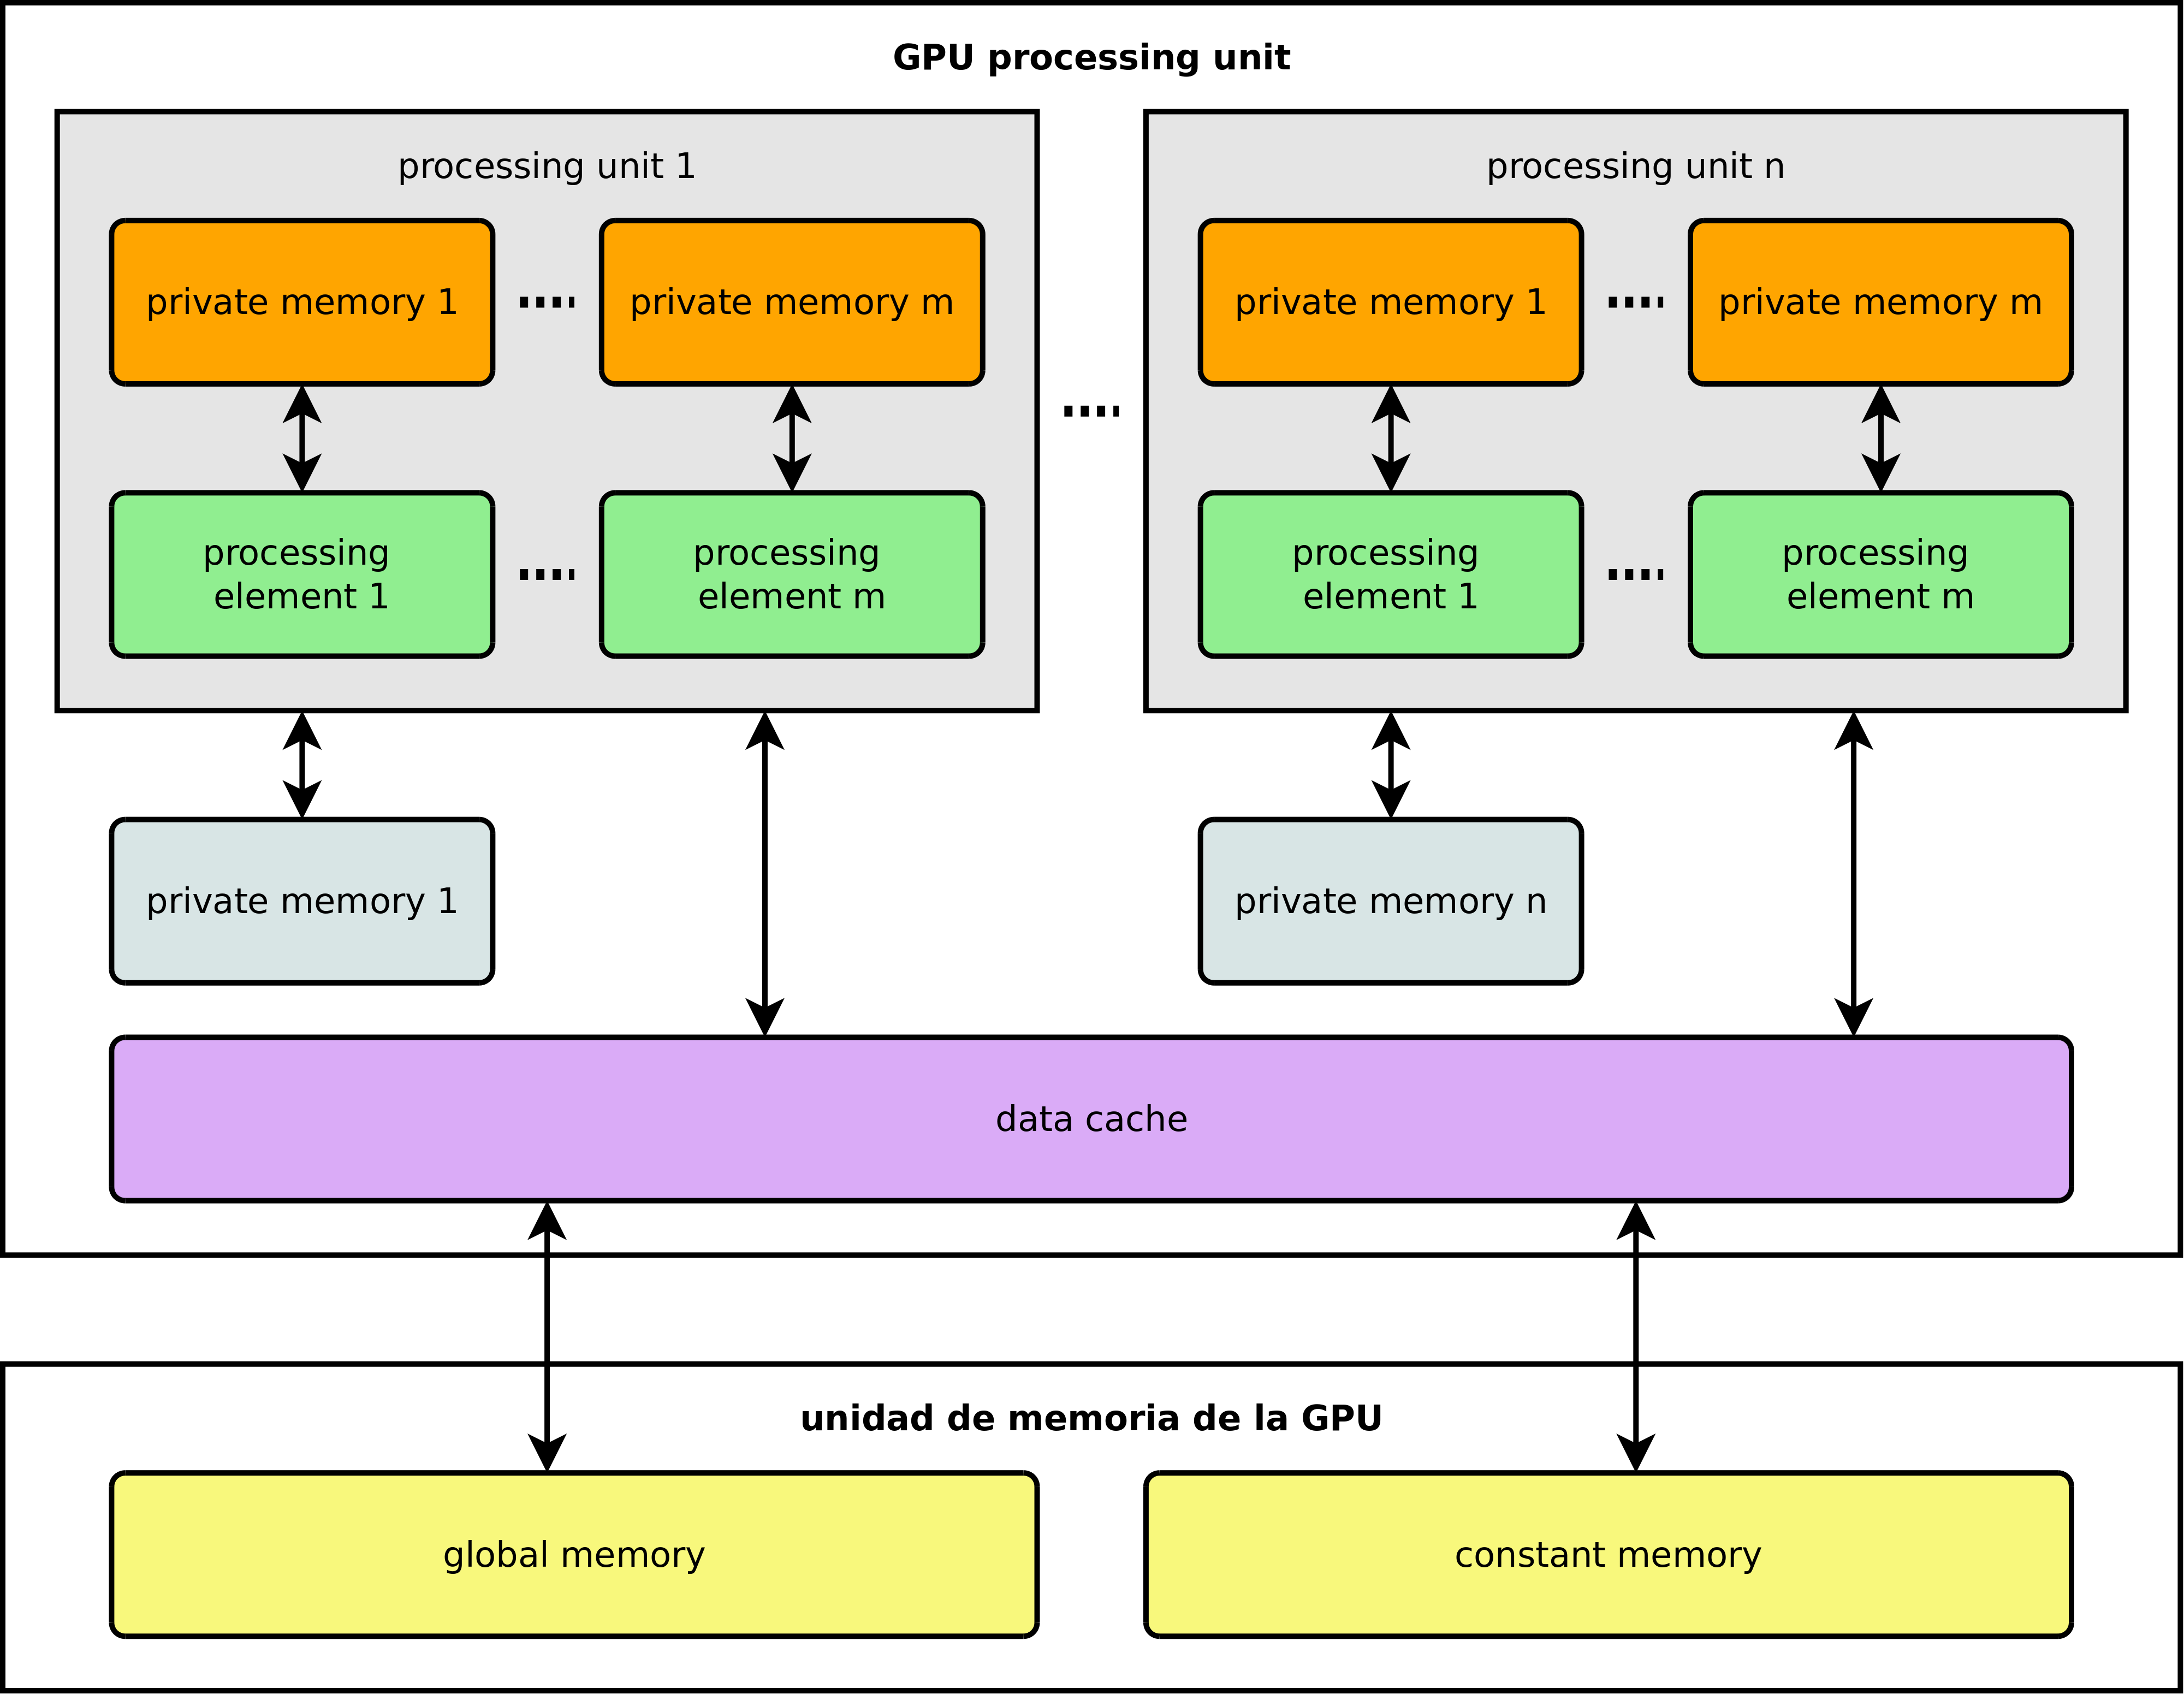
\includegraphics[width=0.9\textwidth]{memory}
\caption{The memory model defines how data is stored and moved between
  CPU and GPU. Global memory is RW (read-write) for both CPU and
  work-items; constant memory is RW (read-write) for CPU and RO (read-only) for work-items; private memory is RW for a single work-item; local memory is RW for a work-group.}
\label{figure:memory}
\end{figure*}

\begin{itemize}
\item Global memory: any work-item and the host CPU can read and write.
\item Constant memory: any work-item and the host CPU can read this read-only region. Writing is only allowed to the CPU.
\item Private memory: a single work-item can read and write from it and is inaccessible for the host CPU. Most computation should be done here because it is the fastest one and the most critical in terms of performance.
\item Local memory: a single work-group can read and write on it and is inaccessible for the CPU. Its main target is to share data between a limited number of work-items.
\end{itemize}

The need to move data in and out of the GPU memory is very common; it
will happen when a calculation is started or when results are
gathered. If the bandwidth consumed by this process involves an
excessive amount of time the target speedup can be ruined. Data
movement should be avoided or at least minimized. This bandwidth
problem has arisen many times in the computation field.

Every time a new powerful device has appear we must feed it data fast enough. Two solutions of recent appearance try to alleviate it. The first is a
fourth level of cache between the CPU and the GPU (or an optimized version of third level one) \cite{Li_EAR_2017}. 
This is only useful when both processors are glued together in the same chip or
encapsulation. The second solution involves changing the way we access
memory from GPU and its called Heterogeneous System Architecture
(HSA) \cite{mukherjee2016comprehensive}. 
HSA shares data between CPU and GPU in a seamless way, avoiding
as many memory copies as caches permits. This way both devices can
share a common memory architecture. Moreover HSAIL is emerging nowadays, in which an intermediate code is used in order to ease the communication process.


%%%%%%%%%%%%%%%%%%%%%%%%%%%%%%%%%%%%%%%%%%%%%%%%%%%%%%%%%%%%%%%%%%%%%%%%%%%%%%%
\subsection{Parallelizing metaheuristics on GPUs}
\label{ssec:parallelizing}
%%%%%%%%%%%%%%%%%%%%%%%%%%%%%%%%%%%%%%%%%%%%%%%%%%%%%%%%%%%%%%%%%%%%%%%%%%%%%%%

GPU implementation of metaheuristics face the same problems as the
implementation of any other kind of algorithm, such as graph
algorithms \cite{shi2018graph}, in these architectures. GPUs work the best when a single
instruction can be applied, in parallel, to a data set; however, CPUs
work better with sequences of computations where the results of one
step are used in other steps. Additionally, GPUs have many more
threads than current CPUs, and needs to be leveraged
\cite{cheng2019accelerating} and is probably more suitable for
fine-grained approaches such as cellular evolutionary algorithms \cite{yu-parallel-2005} or
other non-standard approaches \cite{DBLP:conf/gecco/PospichalMOSJ11}. On the other
hand, CPUs and GPUs must work together, with GPUs needing to access
the computer memory, or the CPU transferring data to the GPU. This
data preparation or data access step is a bottleneck for the full
parallelization of algorithms in GPUs.

It would be ideal, thus, that a framework abstracted this step and
took care of splitting GPU and CPU work along the lines that would
maximize performance. These frameworks would put a layer of
abstraction over the specifics of GPU 
programming, and help practitioners focus on solving the problem
instead of implementing it in a GPU. However, in practice there's no
such thing as a general purpose metaheuristic framework that works on
GPUs. Libraries for  making this implementation a bit easier come in
two different flavors: specific versions of general-purpose
metaheuristic libraries, and frameworks for some specific
metaheuristic that work over GPUs.

In the first case fall library
extensions to frameworks that perform evaluation of individuals,
normally the dominant part in most metaheuristic implementation, in
GPUs.  Robilliard et al. \cite{RobilliardECJGPU08} did it
for ECJ, and Cano et al. for jCLEC
\cite{SpeedingTheEvaluationofGPCano:2012}.
On the other hand, ParadiseEO-MO-GPU \cite{MealbParadiseoGPU13},
another framework built upon an existing one, for now is only focused
in single solution metaheuristics, and it does not support
population-based ones, such as EAs. EASEA
\cite{Maitre:2009:CGP:1569901.1570089} takes a code generation
approach that sends  the code for the fitness
evaluation to the GPU to be run in parallel, so the parallelization
just affects to a part of the algorithm.

The only general purpose EA library that seems to be available is
libCudaOptimize \cite{nashed2012libcudaoptimize}, although it does not
seem to have been updated since 2015. With this library, written in
C++ and CUDA-C, you can either use the framework with your own fitness
function, or implement new optimization methods that leverage que
power of the CPU. As its name implies, it relies on nVidia hardware,
but is able to use as many threads are available without the direct
intervention of the programmer. This kind of framework, however, does
not seem to have had a continuity or been superseded by a new, and
actively maintained, one.

In the second case there are a few examples; PUGACE \cite{5586286} is
one of the few new frameworks focused exclusively on the execution of
EAs in GPUs. It is based on MALLBA and uses CUDA to execute cellular
GAs (cGAs), but only for linear neighborhood structures. However, this
framework does not seem to be available either as open source or any
other form, so it is difficult to check their claims or even use
it. gpuMF \cite{roberge2015gpumf} implements island-model
metaheuristics, and seems to be addressed at generic population-based
models, including GAs and PSOs but not other paradigms, such as GP or
ACOs. As in the case above, it does not seem to be published
anywhere, which implies that only the authors have used it in
publications.

That means that, in general, metaheuristics in GPUs will have to
either use general-purpose open source frameworks and adapt a part of
them for working in GPUs or else roll out your own. In any case, you
will have to take into account a series of constraints, about which we
will talk about next.



%%%%%%%%%%%%%%%%%%%%%%%%%%%%%%%%%%%%%%%%%%%%%%%%%%%%%%%%%%%%%%%%%%%%%%%%%%%%%%%
\section{Literature analysis and review}
\label{sec:survey}
%%%%%%%%%%%%%%%%%%%%%%%%%%%%%%%%%%%%%%%%%%%%%%%%%%%%%%%%%%%%%%%%%%%%%%%%%%%%%%%

In this section we present a quantitative analysis of published papers
on EAs on GPUs. Then, the most relevant ones are classified following a taxonomy similar to the aforementioned schemes for parallel and distributed EAs.

Firstly, an in-depth analysis of the existing related literature has been done. In order to conduct this analysis we performed the query ``\textit{(GPGPU OR GPU) AND (GENETIC OR EVOLUTIONARY)}'' in the Web Of Science (WoS) \cite{wos} database, referred to any part of the publications, and just enclosed into {\em Computer Science} research area.
% Antonio - comprobar si se busca en cualquier parte de los art�culos
% Check out these comments - JJ
% Antonio - Revisar que esta sea la cadena de b�squeda que se ha usado en los �ltimos sondeos.
It yielded 329 references, from which we eliminated those references unrelated to the scope of this paper (for example, those whose topic is related with genetic engineering and not with genetic algorithms). After that removal, 194 results remained, which were carefully read in order to extract its features and useful information for this survey.

Looking at the publication rate per year inside this scope, it can be noticed in Figure \ref{figure:publications}, that the publication figures has been increased every year, starting from 2004, being nowadays a very appealing and prolific field for researchers  (according to the results).

\begin{figure*}[!ht]
\centering
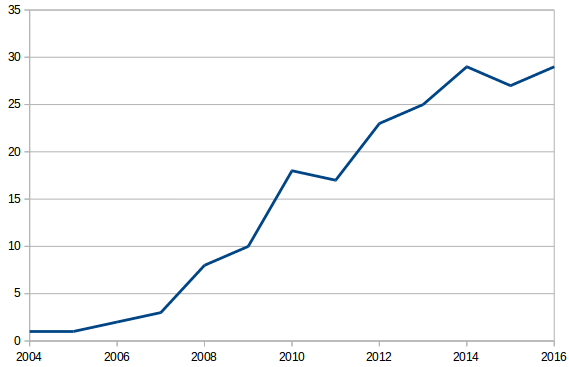
\includegraphics[width=0.75\textwidth]{years}
\caption{Papers published per year in the scope of EAs on GPUs, according to Web of Science database.}
\label{figure:publications}
\end{figure*}


Regarding the type of EA implemented or studied in those papers,
Figure \ref{figure:type_algorithm} shows the percentages of the
different approaches. The most prolific ones are GAs, since it is the
classic optimization method inside EAs. It is easy to implement and
usually yields very good results.  GP and DE are more specific and
thus, less extended or used. `Others' refers to EAs such as EDA
(Estimation of Distribution Algorithm), SGS (Systolic Genetic Search)
or MA (Memetic Algorithms), to cite a few.  

\begin{figure*}[!ht]
\centering
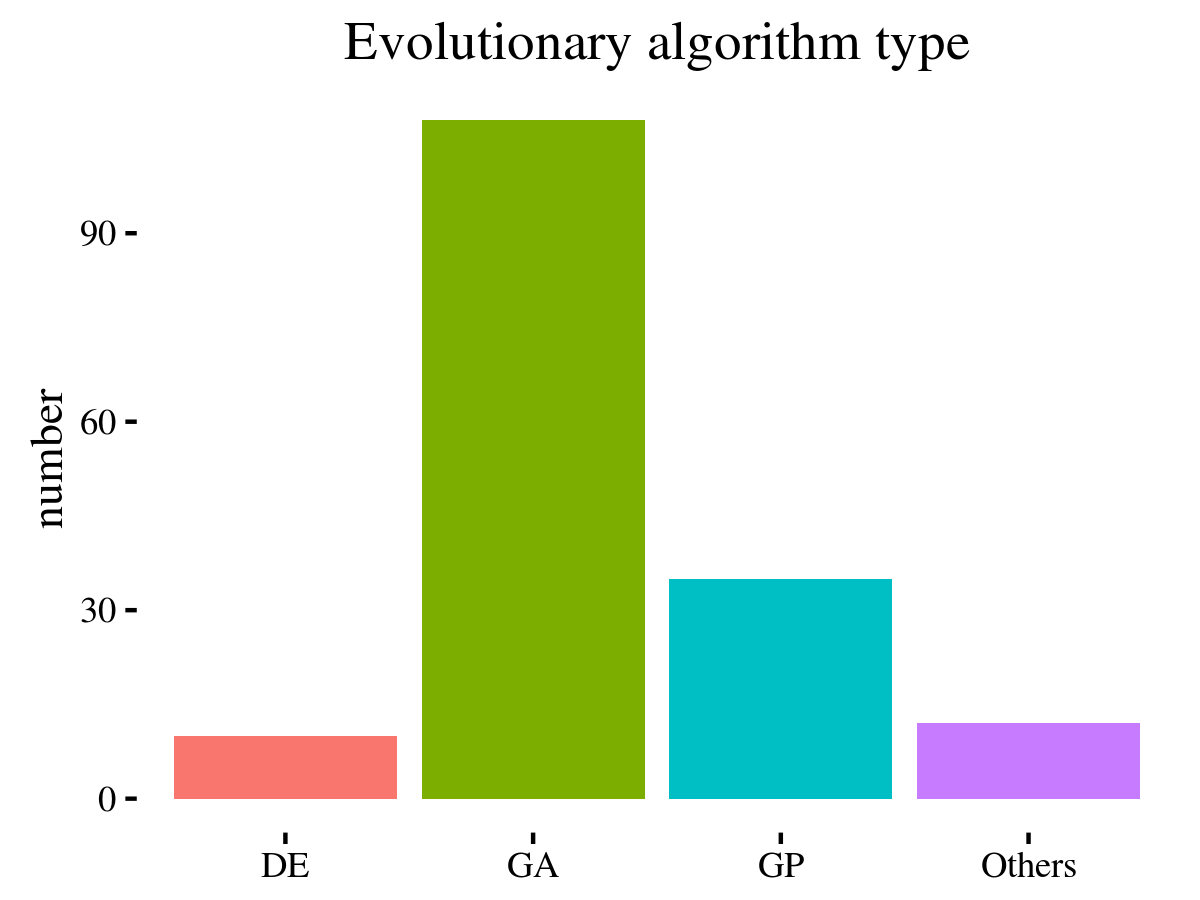
\includegraphics[clip,width=0.7\textwidth]{algorithmtype}
\caption{Type of Evolutionary Algorithm implemented in the analyzed publications.}
\label{figure:type_algorithm}
\end{figure*}

Once analyzed the whole literature from a general perspective, the following sections will go through each of the different groups of the proposed taxonomy. Then, each of the most representative or relevant works (mainly according to their number of citations) are reviewed and commented.

%After reading this section it is clear than PEAs is an active research field and there are so many different variations that almost for sure one of then can fit the needs of most users. Following this reasoning, in the next 5 sections, the most representative works of every type of EA are going to be presented for your convenience.

%%%%%%%%%%%%%%%%%%%%%%%%%%%%%%%%%%%%%%%%%%%%%%%%%%%%%%%%%%%%%%%%%%%%%%%%%%%%%%%
\subsection{Server-client approaches}
\label{sec:serverClient}
%%%%%%%%%%%%%%%%%%%%%%%%%%%%%%%%%%%%%%%%%%%%%%%%%%%%%%%%%%%%%%%%%%%%%%%%%%%%%%%

As a GPGPU implementation, the GPU is responsible for fitness
evaluation but it does not get involved with other phases of the
algorithm such as crossover, selection or even population ranking for
the next generation. In this approach, every generation the
individuals are copied to the global memory of the GPU, so every
single processor gets one or more individuals from global memory and
puts them into the shared memory, in order to decrease global memory
overhead. After that, each thread evaluates it or them, and stores the
result into the global memory again. Usually each single core
evaluates one individual. The programmer has to minimize the number of
global memory accesses, as well as to minimize data transfers between
CPU and GPU. Some additional problems might be faced, like for
example, individuals that require additional data for being evaluated,
such as a distance matrix or a data set. This additional information
might be copied from CPU to GPU once at the beginning of the process,
so the threads might access this data for evaluation minimizing CPU/GPU
traffic.

% Unify using EC or Evolutionary Computation through the paper - JJ
% Antonio - done (it was just used here)
One of the first proposals for parallel Evolutionary Algorithms using
a GPU was done by Wong et al. \cite{man-leung-wong-parallel-2005}. They presented an Evolutionary Programming (EP) algorithm
% without crossover EP does not have crossover - JJ
% Antonio - we said this in the description of EP
% EP is not included in the list of algorithms - JJ
% Antonio - It is.
for solving five simple test functions, called Fast Evolutionary Programming
(FEP). In this client-server approach, some actions such as the main loop of the algorithm were executed in the CPU, while evaluation and mutation were run within the GPU device because both steps do not need of external information exchange. In this case, the reproduction process implies interaction among, at least, two individuals so the authors eliminated this step in the algorithm. A maximum speedup of $\times5.02$ was obtained when the population size increases. This is the most common organization in GPU implementations, since no
interaction among individuals is required during the evaluation, so
this process can be fully parallelized. In that paper the individuals
was real-coded and the genomes were mapped into the texture
memory. Each GPU thread evaluated one individual and returned its
fitness at the end of the parallel process to the CPU, for the next
evolution cycle.

A Genetic Programming (GP) method proposed by Harding and Banzhaf \cite{4215552} is another example of execution of the EA using the GPU for fitness evaluation, while the rest of the steps are executed on the CPU. In this paper real-coded expressions were tested in up to 10000 nodes, boolean expressions in up to 1500 nodes, and some expressions of real world problems in up to 10000 nodes. Results yielded a speedup of thousand times in some instances.
Besides, Chitty et al. \cite{Chitty2016} proposed different techniques to improve the performance of a graphics card implementation of tree-based GP in order to better exploiting this faster device. Authors demonstrated that both L1 cache and shared memory need to be considered for obtaining the maximum performance.

Hierarchical parallel GAs have been adapted using other models. 
For example, Zhang et al. \cite{ZhangImplementationserverClient},
proposed the use of {\em deme} model at high level, and a
client-server schema at low level. In this case, the CPU initializes
the population and distributes the individuals to thread blocks in
shared memory. Then, the GPU threads within each block run a GA
independently, by applying selection, crossover, mutation and
performing the evaluation; and it migrates individuals to other thread
blocks in its neighborhood. However, no speedup results were reported
in this paper. 
On another hand, Djenouri et al. \cite{Djenouri2017a} propose using bio-inspired approaches (GA, PSO, and BSO) to solve well known large association rules mining instances; in their work, after the generation of the rules on CPU, all the obtained rules are sent to the GPU for the evaluation process. In a further works \cite{Djenouri2017b,DJENOURI2018}, an intelligent strategy is proposed to partition the search space of rules in several independent sub-spaces to allow multiple CPU cores to explore the search space efficiently and without performing redundant work, having obtained that the suggested approach outperforms the sequential version by up to at 600 times for large datasets. 

In \cite{Jurczuk2017}, authors design and implement a graphics processing unit (GPU)-based parallelization of evolutionary induction of decision trees; in this method the selection and genetic operators are performed sequentially on a CPU, while the evaluation process for the individuals in the population is parallelized on GPU.
A similar approach has been proposed by Vidal et al in
\cite{Vidal2017}, where authors propose a hybrid CPU-GPU
implementation on multi-core CPUs plus a GPU using OpenMP and CUDA
respectively; in this method, the solutions of the CPU technique are
used to replace some of the solutions in the GPU algorithm.

Van Luong et al. \cite{5586403} published in 2010 a methodology for mapping the search space onto the GPU memory hierarchy in three levels: (1) the distribution of the search process among the CPU and GPU, (2) the mapping of the neighborhood in the GPU threads, and (3) the effective usage of the texture memory in the context of hybrid EAs. Experiments to solve the QAP problem with CUDA were presented, where the evolutionary process was performed in the CPU and the generation of the Local Search neighborhood were conducted on parallel in the GPU, achieving an acceleration of $\times14.6$ times faster. Hardware used was Core 2 Duo 2.67GHz and nVidia GTX 280. This work also showed the benefits of using a conjunction of CPU + GPU, being the GPU used only for intensive calculations.

There are papers related with other lines, like \cite{Pedemonte:2011:BOG:2001858.2002031} which studies the
impact of using different representations for binary problems in GPUs
to evaluate GAs: boolean data type versus packing multiple bits in a
non-boolean data type. The execution platform was a PC with a Quad
Core Intel Xeon E5530 processor at 2.4GHz and a Tesla C1060 with 240
CUDA cores. The CPU only calculates the initial population and a
matrix of random numbers to be used in crossover and mutation by the
GPU. The authors reviewed the problem of the data types when GPUs are
used. Several data types of 8, 16, 32, and 64 bits are compared in CPU
and GPU versions. Results showed that packing in 32 bits data types
achieve speedup values of up to $\times100$ compared with boolean data
types, specially when the size 
of the instances increases. This make sense because the Tesla C1060
are equipped with 32-bit integer ALUs.

Cano et al. \cite{SpeedingTheEvaluationofGPCano:2012} described a massively parallel evaluation model using a Genetic Programming algorithm for evolving rules for dataset classification. They copied the dataset to the GPU global memory, and evaluated the rules (individuals) for each instance of the dataset in parallel (match kernel). At the end, each successful match was reduced getting each individual fitness (reduction kernel). The implementation, based on CUDA, speedups the fitness calculation phase and greatly reduce the computation time. Results were compared using one, two and four CPU threads and the combination of one or two GPUs of different features (285 cores for GPUa -nVidia GeForce 285 GTX- or 480 cores for GPUb -nVidia GeForce 480 GTX-). They test three classification algorithms and the results were not very significant for small datasets, but they increased the speedup with large datasets until $\times820$ using two GPUs with 480 cores each one.

The work by Chitty \cite{Chitty16FastParallel} uses a client-server architecture for evaluating at time the population for four GP problems. The results were achieved using an nVidia GeForce Kepler 670 GTX graphics card and compared with a previous one-dimensional stack approach for the same problems. The author fit the algorithm until to observe a peak computational speed of over 55 billion Genetic Programming Operations per second a twofold improvement over the previous one-dimensional stack approach.


Recent works are currently being applied to real-world problems. Jaros et al. \cite{Jaros14Wormhole} use GPUs to lower the run time and improve the quality of the solutions in the problem of wormhole switching in collective communications. The start from an evolutionary tool capable of finding optimal communication schedules for various communication patterns on wide range of interconnection networks topologies of up to 256 nodes. The tool consumes tens of hours so they decide to improve it. As the fitness evaluation was responsible for the 93\% of the execution time this was the only part moved to the GPU. In a first step only one GPU was used with speedups up to $\times5$. After that they made a new implementation capable of using 8 GPUs and 30 times faster than the original.
Rey et al. \cite{Rey2018} presented a new hybrid approach based on Ant Colony Optimization heuristics, Route First-Cluster Second methods and Local search procedures, combined to generate high quality solutions for the Vehicle Routing Problem. Authors propose the parallelization of the whole algorithm through a heterogeneous CPU-GPU implementation.

In \cite{Contreras:2012:UGA:2150467.2150469} the authors use a CPU-GPU architecture for stock market trading. The proposed architecture offers the benefices of GPU distribution for stock market researchers, rather for computer architecture experts. The authors used Jacket \cite{jacket:Matlab}, a software platform for the rapid development of GPGPU computing applications within the MATLAB computing environment, C, and C++. However, this framework is no longer available \footnote{\url{http://blog.accelereyes.com/blog/2012/12/12/exciting-updates-from-accelereyes/}}. Steps and guidelines to migrate from CPU code to GPU code are explained, what is a great contribution, because usually, the authors do not include this information in the papers. The algorithm run in the CPU, but all  {\em for} loops in selection, evaluation, crossover and mutation are translated to Jacket's {\em gfor} to be parallelized in the GPU. Three different CPU configurations are used for the experiments: Pentium 4, Pentium SU41000 and Intel Core i7-860. The former is also combined with an nVidia 460GTX for GPU experiments. Different population size are also tested. The time is reduced to 65\% in comparison with the CPU version. Other conclusions are obtained: speedups with high number of individuals, rather than increasing the number of evaluations; and time reduction for  tournament selection  over roulette-wheel selection.

Stock market trading analysis has also been recently addressed by
using GP in GPUs. The algorithm described in the work by Sungjoo et
al. \cite{Sungjoo15fastknowledge} is used to solve the problem of
knowledge discovery in stock market time series, i.e. finding the
so-called precursor patterns, which model events occurred in the time
series. Thus, every individual (tree) in the GP algorithm is a
pattern, which must be matched against the whole dataset to find
out if it is a precursor. This is what the evaluation function
does. The time series is divided into different subsets, and stored in
several GPUs. The data is then copied once and just the new
individuals to evaluate and the partial results of the evaluation must
be transferred and updated, avoiding bandwidth problems.
The run is conducted for 50 generations and with 500 individuals of a maximum depth of 3 levels, using a i7-3820 CPU and 8 CUDA GPUs (GeForce GTX 690).
% You need to give that amount of details? - JJ
% Antonio - This is usual in CPU-GPU papers in order to compare the computational power when the speedup is calculated.
The authors considered
512 threads per block, 260 blocks per grid and just one grid per
GPU. The comparison in performance yields a reduction of 56 times for
just one GPU to 277 using all of them. This improvement is obtained using
local memory allocation, using the shared memory of blocks instead
yields a smaller improvement of around 188 times faster in the best
case. Regarding the influence of individuals' tree size (number of
nodes) in the performance, the authors show that the running time
grows for just one GPU, but when more than four are used, this growing
is minimum and could be assumed in order to improve the quality of the
results. % Some comment with respect to bandwidth? - JJ


%%%%%%%%%%%%%%%%%%%%%%%%%%%%%%%%%%%%%%%%%%%%%%%%%%%%%%%%%%%%%%%%%%%%%%%%%%%%%%%
\subsection{Fine-grained Approaches}
%%%%%%%%%%%%%%%%%%%%%%%%%%%%%%%%%%%%%%%%%%%%%%%%%%%%%%%%%%%%%%%%%%%%%%%%%%%%%%%

Researchers implement fine-grained algorithms using GPUs, making
every scalar processor (SP) to evolve an individual. This individual
interacts with other SPs that belongs to the same Streaming
Multiprocessor (SM) to perform the basic operations of the algorithm
like crossover or mutation. In this approach a big part of the
algorithm runs within the GPU and not only the evaluation phase like
in previous section (\ref{sec:serverClient}). The GPU architecture
assists the neighborhoods emerge since each group of SMs have a shared
memory, where SPs access without penalty. The exchange of information
between individuals through this shared memory is
inexpensive. However, programmers have to be careful with the
information exchange between individuals in different SMs.

The second problem of this approach is the random number
generator. The CPU can easily generate random numbers, but the GPU is
not able to do this task.
So researchers have to think about how to solve this problem. Usually the algorithm's implementation generate at the beginning a big set of random numbers and they are copied to the GPU as a list. After that, the GPU uses the random list when needed and when it need. This approach saves time for random generation but the list of random numbers has to be limited. Moreover, all SPs could use the random numbers, so the list must be available for every
thread.


Yu et al. \cite{yu-parallel-2005} implemented the first real cellular EA using GPUs, for solving the Colville problem \cite{Ng:2005:DFF:1064290.1064296} in 2005. The population is distributed in a toroidal 2D grid and the classical Von Neumann neighborhood structure with five cells was used. Chromosomes and their fitness values were stored in the texture memory on the graphic card, and both, fitness evaluation and genetic operations, were implemented entirely with fragment programs executed in parallel on GPU. Real-coded individuals were represented as a set of 2D texture maps. BLX-$\alpha$ crossover and non-uniform mutation was developed as tiny programs on every pixel at each step in a SIMD-like fashion. They solved some optimization problems and reached a speedup of $\times15$ with a population of 512x512 individuals. They store a set of random numbers at the beginning of the evolution process to solve the random number generation problem when using GPU processors.

In 2006, \cite{man-leung-wong-parallel-2006} proposed a parallel hybrid GA (HGA) where the whole evolutionary process run on the GPU, and only the random number generation is done in CPU. Every individual is assigned to a GPU thread, and each one selects probabilistically an individual in its neighborhood to mate with it. Just one offspring individual is generated each time, and it replaces the old one in that GPU thread. The authors compare their implementation with a standard GA run in a CPU and the FEP \cite{man-leung-wong-parallel-2005} algorithm. Using a new pseudo-deterministic selection method, the amount of random numbers transferred from the CPU is reduced. HGA reaches speedup of $\times5.30$ when compared against the sequential version. In 2009 Wong et al. \cite{wong-implementation-2009} provide implementation details for fine-grained evolutionary algorithms.

Liu and Luo \cite{zhongwen-luo-cellular-2006} implemented a cellular algorithm on GPU to solve three different satisfiability problems (SAT)
using a greedy local search (GSAT) \cite{Selman93domain-independentextensions} and a cellular GA (cGA).
They saved local minimums using a random walk strategy, jumping to other search space location.
The cellular GA adopts a 2D toroidal grid, using the Moore neighborhood, stored on texture GPU memory. This implementation generates the random numbers in the GPU (using a generated seed on the CPU at the beginning of the process). They carried out the experiments using two GSAT implementations, CGSAT (with crossover and without mutation) and PGSAT (without crossover and with mutation) running them on CPU and GPU with different population sizes. A great time reduction was reached using the GPU parallelization approach (from 95ms to 18 ms for CGSAT and from 464ms to 77 ms for PGSAT).

Li et al. \cite{jian_ming_li_efficient_2007} proposed a cellular algorithm on GPU for solving some common approximation functions. The authors reported experiments using big populations (up to 10000 individuals) reaching speedups of $\times73.6$ for some implementations. The novelty of this paper is the bit dataset because it is not easy to deal with bit datasets using a GPU due to the memory size restrictions. The GPUs does not support binary operations, but in this paper the authors dealt with binary individuals of 24 bits  and simulated bit-operator by judging each bit of a binary value is 1 or 0. They faced a general problem for all GPGPU community with bit operations. They proposed to use random-textures for random numbers generation, but the random numbers were generated on CPU previously.

As in previous work, fitness evaluation and genetic operators were applied in the GPU by Gonz\'alez et al. \cite{springerlink:10.1007978-3-642-12538-619} by using CUDA, and storing individuals and their fitness values in the GPU global memory.
The difference is that they used a pseudo random number generator provided by the SDK of CUDA named Mersenne Twister. Some general discrete and continuous optimization problems were used in the experimental setup, and physical and numerical efficacy were compared with respect to CPU implementation.

In \cite{Li:2009:PIA:1726585.1726930} the authors proposed an Fine-grained parallel immune algorithm (FGIA) which is an Artificial Immune System combined with an EA. Three medium-size instances of the Travelling Salesman problem (TSP) were solved by using a fine-grained parallel algorithm with CUDA C. The algorithm enlarges the population size of FGIA maintaining better population diversity. As a remark, the authors included a sub-linear relation between the population size and the execution time, which made the proposal very useful for solving difficult problems that require huge population sizes.

Depending on the problem size, fine-grained approaches may improve the
efficiency with respect to the coarse-grained version. For example, in
the work of Franco et al. \cite{Franco15LargeScale}, two different
approaches for strategies for GPU implementations of the evaluation
stage of evolutionary rule learning are analyzed and the types of
problems where each method performs best have been identified. The
coarse-grained implementation is more conservative and only
parallelizes the evaluation of instances, while the fine-grained
implementation expands the parallelism to the attribute dimension and
is faster on data sets with 10 to 50 discrete attributes.


%%%%%%%%%%%%%%%%%%%%%%%%%%%%%%%%%%%%%%%%%%%%%%%%%%%%%%%%%%%%%%%%%%%%%%%%%%%%%%%
\subsection{Coarse-grained approaches (Island Model)}
% why mix caps and not? - JJ
% Antonio - fixed
% This is the same structure as the 2012 paper. It should be updated. 
%%%%%%%%%%%%%%%%%%%%%%%%%%%%%%%%%%%%%%%%%%%%%%%%%%%%%%%%%%%%%%%%%%%%%%%%%%%%%%%

The coarse-grained algorithms are the most common among parallel EAs, as mentioned in Section \ref{subsec:coarsegrainedapproaches}, due to the inherent parallelization possibilities they offer. Thus, these algorithms require less tightly coupled parallel architectures, as compared to fine-grained ones.
This kind of EAs works by dividing the main population into sub-populations (also known as `islands') which evolve concurrently, and from time to time, some individuals are moved from one island to another (migration).
This basic feature of coarse-grained EAs hits a physical limit of
GPUs.

In order to run a coarse-grained EA using a GPU device, several kernels could be run simultaneously. In that case, each kernel could handle a sub-population of individuals, establishing some synchronization points.
However, the GPU architecture is not designed for synchronizing
different kernels into the same grid, which means that using a GPU to
run a coarse-grained EA might require changing some standard mechanisms
of the algorithm.


One of the first island models on GPU-based approaches was presented on the GECCO 2009 GPU Competition \cite{gecco2009CompetitionPospichal}. This technical report presented some technical details of an island model entirely hard-coded on GPU, with a ring-neighborhood topology. As it was a first attempt, the evolutionary operators implemented on GPU were only specific to the GECCO competition, and the validity of the experiments is not clear, since the approach just worked on a small number of problems.

However, after this, Pospichal et al. continued working on their approach \cite{pospichalParallelGeneticAlgorithOnCUDA2010,9253}. The authors mapped threads to individuals, and then, these threads-individuals could be synchronized easily in order to maintain data consistency. To decrease memory latency, the usage of an on-chip hardware scheduler was proposed, which swiftly swaps existing islands between multiprocessors, with the combination of a fast-shared memory. In this case, the population size was limited to 16KB per island (as on most GPUs at that time), so if the population was larger, the main memory would be used, implying a time increase. In fact, the inter-island communication was used, by relying on it the migration, based in an asynchronous unidirectional ring model. Even that, authors reported speedups up to $\times7000$ times higher on GPU compared to CPU sequential version of the algorithm.

Permutation domain problems have been studied by some authors. Tsutsui
and Noriyuki \cite{1570355} also run a coarse-grained GA on a GPU,
to solve the QAP problem using CUDA. Their model generated the initial
population on CPU and copied it to the GPU VRAM; then, each
sub-population in a GPU (nVidia GeForce GTX285) was evolved. At some
generations, individuals in sub-populations were shuffled through the
GPU VRAM. Results showed a speedup from $\times3$ to $\times12$ (using
eight QAP instances), in the comparison with an Intel i7 965
processor. 

Comparison of several approaches is a very important task to do when presenting a new model. The work by \cite{LUONG:2010:INRIA-00520464:1} compared three different schemes, including his new re-design of the island model. The first scheme presented implemented a coarse-grained EA based on a client-server model to run the evaluation step on GPU, as other papers mentioned early. The second one directly distributed the EA population on GPUs. Finally, the use of a fast on-chip memory was proposed as an extension on the third approach.
The two latter approaches reduced the CPU-GPU memory latency, although their parameters (number of islands, migration topology, frequency, and number of migrants) must be adapted to the GPU features. Sequential and parallel implementations were compared, obtaining a speedup of $\times1757$ using the third approach.


The coarse-grained models are still being investigated. Recently, Li
et al \cite{Li2016} developed a parallel GA for GPUs. They took
advantage of the many cores of GPUs to enhance computation efficiency,
by using a large amount of threads simultaneously. This strategy
allows the population to scale and accelerates the speed to find the
global optimal solution. Zhengfu et al. \cite{Zhengfu2016} proposed to
improve the computational efficiency of information entropy
multi-population GA, and to reduce the computing time, by using a
CUDA-based implementation. 


%%%%%%%%%%%%%%%%%%%%%%%%%%%%%%%%%%%%%%%%%%%%%%%%%%%%%%%%%%%%%%%%%%%%%%%%%%%%%%%
\subsection{Hierarchical Models}
%%%%%%%%%%%%%%%%%%%%%%%%%%%%%%%%%%%%%%%%%%%%%%%%%%%%%%%%%%%%%%%%%%%%%%%%%%%%%%%

As mentioned before, these approaches aim to combine previous models,
in order to take advantage of the best of every one, for instance,
fusing the client-server evaluation with the diversity mechanisms of
island-based models. 

This is the case of the work by Munawar et
al. \cite{Munawar:2009:HGA:1666141_1666143}, where the design and
implementation of a hybrid EA with local search to solve MAX-SAT over
GPUs was thoroughly discussed. The authors implemented a hierarchical
algorithm of 2D structured sub-populations arranged as islands in a 2D
grid. Thus, every individual and sub-population has 4 neighboring ones
(north, south, east and west). A new technique called {\em diffusion}
is used instead of a conventional algorithm for the migration between
sub-populations, as it is more suitable for the implementation of cGAs
based pGA over a GPU. In the proposal, the host processor (CPU) acts
as a controller, while a nVidia Tesla C1060 GPU provides the required
computational resources. This processor is also responsible of
configuration, memory allocation and initialization. After the
initialization stage, data is transferred to the device and the code
enters a loop. The loop keeps on repeating until the maximum number of
generation criteria is satisfied. Results were collected over a system
with nVidia Tesla C1060 GPU mounted on a motherboard with Intel Core
i7 920 2.67GHz as the host CPU. C1060 have 4GB of device memory, 30
streaming multiprocessors, and the total number of processing cores is
240. The maximum amount of shared memory per block is 16KB and clock
rate is 1.30GHz. They compare the results of the algorithms over
nVidia with optimized for local search, mutation, recombination,
selection and diffusion (migration) with different implementations
using serial implementation, OpenMP implementation over Intel and over
UltraSPARC architectures. The found that the maximum speedup is for
larger problems, and it is up to $\times25$ if compared the serial
implementation over Intel Core 2 Duo 3.3GHz with the nVidia
implementation. 

%Diego et al. \cite{fjdiego-vrp}proposed a parallel strategy for solving the Capacitated Vehicle Routing Problem (CVRP) by means of an ACO algorithm. They combined the CPU processing, random number generation and centralized pheromone information dealing, with the GPU parallel capabilities: initialization of trails, build solutions, choosing of the best solution, and pheromone evaporation. The experiments were conducted on a GeForce GTX460 in a Pentium Dual Core 2.7GHz with 2GB RAM, using CUDA. The results showed a speedup of $\times12$ in the best case.

%Cecilia et al. \cite{Cecilia201342} proposed three different techniques for improving the classical ACO algorithms parallelization on GPUs: a data parallelism scheme for tour construction on GPU, a GPU-based pheromone updating stage, and a roulette wheel implementation on GPU, called I-Roulette. They introduced the queen ants, associated with CUDA blocks, and the worker ants, associated to CUDA threads. The experiments were performed on a four-core Intel Xeon E5620 running at 2.4 GHz, with 16GB RAM, and a nVidia Tesla C2050 Fermi. The proposed techniques lead to obtain a speedup factor of up to $\times20$ in comparison with the sequential implementation.

In \cite{5586530} three cellular GA versions are compared: a CPU, a mono-GPU and a multi-GPU version, being the first work in use multi-GPU for cEAs. A 2D grid population is used and divided in two GPUs in the multi version. Selection, recombination, mutation and evaluation are performed in parallel. In the multi GPU case, a thread for each GPU is controlled by a CPU thread and borderline individuals of the sub-populations are exchanged. The speedup ranges from $\times8$ to $\times711$. However, there is not significantly difference between mono and multi GPU versions, probably due the overhead of the CPU. Hardware used is Intel Quad processor 2.67GHz and nVidia GeForce GTX 285.

During 2012, Luong \cite{luongMetaheuristicsPpsn2012} implemented a GPGPU algorithm from the metaheuristic point of view. In the paper a guideline to exploit heterogeneous computing resources, including GPU and CPUs, for effective hybrid metaheuristics was proposed. The goal of this paper is not the evaluation of the fitness of some individuals, but the parallelization of metaheuristics which were not inherently parallel, like local search algorithms. Task distribution is clearly defined into the paper, the CPU manages the whole sequential Local Search process and the GPU is dedicated to the costly part i.e. the parallel generation and evaluation of the neighbor solutions.

Authors mapped the population to the GPU and applied the parallel metaheuristic to each individual using its neighborhood structure taking advantage of the blocks of threads present in the GPU architecture. The parallelization of these metaheuristics generated several different individuals that the GPU evaluated at the same time. The critical issue was finding efficient mappings between a GPU thread and a particular neighbor. Indeed, this step is crucial in the design of new large neighborhood local search algorithms for binary problems since it is clearly identified as the gateway between a GPU process and a candidate neighbor. They reviewed neighborhoods based on a Hamming distance of one, two and three, and applied their suggestions to Permuted Perceptron problem \cite{KnudsenPermutedPerceptronProblem1999}. They considered a Tabu Search algorithm \cite{Wu16Tabu} using CUDA for each neighborhood with a configuration of Intel Core 2 Duo 2.67GHz with a nVidia GTX 280 card. The CUDA implementation increased the number of successful solutions drastically every instance of the problem. Regarding execution time, acceleration factors using GPU are very significant (from $\times24.2$ to $\times25.8$).

In 2014, \cite{Wang14heterogeneous} used a supercomputer platform to run a CPU+GPU high performance EA. 16 islands of 8 individuals were set as parameters. The experiments were carried in a combination of Intel Xeon X5650 2.66GHz and  Intel Xeon X7550 2.0GHz processors, although the paper do not includes information about the graphic cards used. Several instances of heterogeneous scheduling problems were used to compared with other metaheuristics, obtaining better makespans.

In \cite{Lin:2016:AGA:2895619.2895696}, an auto-tuning approach based on SA and GA for GPGPU applications taking into account the performance and power models is presented. Thus, no sub-optimal configuration that leads to poor performance and/or high power consumption is used.


%%%%%%%%%%%%%%%%%%%%%%%%%%%%%%%%%%%%%%%%%%%%%%%%%%%%%%%%%%%%%%%%%%%%%%%%%%%%%%%
\subsection{Non-standard Approaches}
%%%%%%%%%%%%%%%%%%%%%%%%%%%%%%%%%%%%%%%%%%%%%%%%%%%%%%%%%%%%%%%%%%%%%%%%%%%%%%%

Pospichal et al. in 2011 has presented several papers related with GPU devices. One of the last is \cite{DBLP:conf/gecco/PospichalMOSJ11} where they propose to use a GPU device for Grammatical Evolution, evolving complete programs in an arbitrary language using variable length binary strings. For this problem, every individual is a program, so it must be compiled and sent to the GPU for being evaluated every generation. However the most time-consuming part of this approach is to sent the individuals to the GPU and not the evaluation itself, so, the authors propose to evolve the whole Grammatical Evolution algorithm on the GPU with a special mapping function. They mapped one individual per block of threads and one thread is used to manage each individual. They compare the execution time of an Intel Core i7 with nVidia GTX 480 using CUDA (CPU implementation with C) an a Java library called GEVA \cite{O'Neill:2008:GGE:1527063.1527066}, which is an interpreted language (CPU implementation using GEVA).  The authors include results for both implementations (C and GEVA) and one GPU implementation, and they compare them with and without overhead for CPU-GPU communication. We include only the results with overhead, because the parallel version needs the CPU-GPU communication, so the authors might take care about it. The results of GPU implementation are in average 5.3 speedup than CPU with C implementation which is an expected result. The speedup grows until $\times102.8$ when GPU implementation and CPU implementation with GEVA are analyzed, but the authors do not include any standard deviation results, so we do not consider the last result as the most important of the paper. Thus, this paper proposes two levels of parallelism: 1) individuals are evaluated in parallel (by threads in the same block); and 2) data within individuals (genes, crossover points, mutations, fitness points, etc.) are maintained by parallel access as well (by block of threads).

Wang et al. \cite{Wang129} proposed a GPU based Neural Network Learning Algorithm based on DE with Improved Elite Strategy. Authors compared the performance with the learning algorithm based on DE with elite strategy running on CPU, resulting that the training time of proposed implementation is shorter while the prediction precision is higher.

Brevilliers et al. \cite{Brevilliers2016} introduce a hybridization of Backtracking Search Optimization Algorithm (BSA) with DE and SA in order to improve the convergence speed of BSA implemented in CUDA. Experimental results show a high performance in terms of solution quality, convergence speed and speedup achieved.

On the other hand, Hwang et al. \cite{Hwang7470556} proposed an EA inspired by biological deoxyribonucleic acid (DNA) computing  to perform the task of optimization. However, to avoid the problems of biological DNA computing and fully utilize parallelism characteristics of it, authors propose to implement the algorithm in a GPU devices, thus optimizing the processing time efficiency.

Finally, due to the complexity of some real problems, several authors have proposed parallel multi-objective implementations on GPU devices, such as Oliveira et al. \cite{Oliveira7744337} who present a GPU-based parallel implementation of NSGA-II to solve the energy dispatch problem of a hydroelectric power plants, taking into account the real time restrictions posed by the operation of a real power plant. The use of a parallel implementation using GPUs improved both the performance and solution quality obtained using the parallel approach.
In \cite{Bian2016} a CPU+GPU heterogeneous computing orientation based
multi-objective test case prioritization technique that utilizes GPGPU
computing to accelerate the process of test case prioritization is
proposed. In this case, the implementation, based on NSGA-II achieves
30 times speed-up rate on a well-known real world problem. 
Manoatl and Coello \cite{ManoatlLopez2016} propose a GPU-based
parallelization of a multi-objective memetic algorithms (MOMAs) which
switches between a hypervolume-based global optimizer and an IGD+
based local search engine for splitting the objective space into
sub-regions. The parallel implementation lead to a high performance
and speedup improvement.

Latest works are based on more complex evolutionary processes, for example, being a step in complex encryption systems \cite{Aljawarneh18Encryption}. Algorithms, such as the SCE-UA, that can be deteriorated performance when dealing with complex models and big data, can benefit from the combination of multi-core CPUs and many-core GPUS. In \cite{Kan17SCEUA} the SCE-UA algorithm was improved by the use of heterogeneous parallel computing. This algorithm is a more complex process of evolution of solutions, being conformed by several steps: combination of probabilistic and deterministic  approaches, clustering, systematic evolution of a complex of points spanning the space, and competitive evolution.

% These non-standard approaches do this or that... - JJ
% this comment still not addressed - JJ

% ---------------------------------------------------------------------

%\section{Comparison with other high-performance methods}
%\label{sec:comparison-hpc}
%
%Some methods to compare with:
%
%\begin{itemize}
%\item Cloud Computing
%\item HP Volunteer Computing    % https://www.arcos.inf.uc3m.es/hipervoco/
%\item FPGAs
%\end{itemize}

% Antonio - I think we shouldn't do this section

% ---------------------------------------------------------------------

\section{Discussion on new trends and future challenges}
\label{sec:discussion}

After reviewing previous papers, new trends can be drawn:

\begin{itemize}

\item Real World Problems: We have observed an increase on the number of papers dealing with Real World Problems. These problems usually imply to deal with massive amount of records and high-dimensional data \cite{Hwang7470556}, or even Real-Time necessities \cite{Maggiani2018}. In fact, new techniques proposed also address other related issues such as filtering, noise-removal or feature selection. Complex models can be leveraged by the use of more advanced optimization techniques, such as the SCE-UA, in combination with multi-core CPU and many-core GPU approaches \cite{Kan17SCEUA}.

\item Big data: Dealing with all these previous issues has led to the emergence of new techniques, mainly the Map-Reduce paradigm. Different works take advantage of the GPU capabilities to deal with large datasets using techniques such as pattern discovery \cite{Djenouri2017b},  ... DeepLearning \cite{Gadea-Girones2018} 

\item Virtualization: % this is not there. 

\item Cloud Computing:


\item Multi-objective optimization: Dealing with more than one optimization objective implies a different way to deal with the fitness calculation. As all the solutions need to be compared to each other to calculate their Pareto Front, traditional parallel schemes need to be adapted in a non-trivial way. Different methods to deal with this issue have been proposed, such as ...

\item Parameter control: Since the origin of the research 



\item Heterogeneous architectures: Even as dozens of low-cost
  Multi-CPU-FPGA can achieve the same performance than a GPU, GPGPU computing is still the best cost-effective solution \cite{Gadea-Girones2018}, so finding techniques to efficiently combine both technologies is the key to outperforms its inherent limitations. Other Hybrid parallelizations, such as MPI/CUDA have also been proposed for further research \cite{Jurczuk2017}. However, a lot of works do not include enough details about the benefits to maximize the usage of CPU-GPU combinations to take leverage the irregularity of data access. Future trends will include new methods related to the improvement of core and cache efficiencies \cite{Escobar17GPUCPU}, or even relaxing on CPU-GPU synchronization to reduce idle times \cite{Rey2018}. 

\item Load balancing: Related with the previous issue, different
  client-server approaches have been proposed, usually distributing
  the evaluation of the individuals among the available threads in the
  GPU. However, new trends involve island-based models... Future
  research is aimed on how to reduce convergence time by managing the
  concurrent pool of solutions \cite{Rey2018} or... % Please add here
                                % - JJ

\item Energy consumption: An important aspect requiring further
  investigation is power consumption, as this issue is becoming crucial
  \cite{Maggiani2018}. Techniques such as power-aware scheduling
  \cite{Escobar17GPUCPU} are being proposed to deal with ...  % Please
                                % add here - JJ

\end{itemize}


Future challenges ...

%%%%%%%%%%%%%%%%%%%%%%%%%%%%%%%%%%%%%%%%%%%%%%%%%%%%%%%%%%%%%%%%%%%%%%%%%%%%%%%
\section{Conclusions}
\label{sec:conclusions}
%%%%%%%%%%%%%%%%%%%%%%%%%%%%%%%%%%%%%%%%%%%%%%%%%%%%%%%%%%%%%%%%%%%%%%%%%%%%%%%

This work has considered the most parallelized and distributed
metaheuristic on the literature, Evolutionary Algorithms (EAs), and
has conducted an exhaustive revision of the existing works, using
General Purpose computing on Graphic Processing Units (GPGPU computing) to implement these
approaches.

The paper gives an introduction to the different existing GPU architectures, physical cards in the market, usual programming languages, and main frameworks, used nowadays in the industry and in this scientific area.
Some guidelines are presented to the reader, in order to point out the main restrictions and issues to take into account when such a parallelization approach wants to be implemented on an EA.

In addition, the work also proposes a novel taxonomy to classify the different types of GPU-based EA parallelization models published, and then, most of the existing papers in the literature have been reviewed, commented and analyzed in a deep and wide survey.
Thus, the work aims to be a reference for future authors, both, from the point of view of its introductory or tutorial use, and also as a compendium of the main proposals in this area, and their characteristics.

The main conclusion reached in this work is also its main justification, as the publication tendency in this field is growing continuously, being in the last three years more than 25 papers on average. 
% Antonio - This was true in 2012, not now unfortunatelly... Rewrite this in accordance of the current tendency.
The main implemented methods are Genetic Algorithm approaches (more than 50\% of the reviewed papers), and around 60\% the publications are focused on solving real problems, taking advantage of the high computational power than GPUs offer to the researchers.

With respect to the most extended programming language, CUDA (for nVidia cards) is the clearly the winner, as it seems to offer better performance and specific tools for the most used cards.

Of course, in almost all the cases, very big speedups are attained in comparison with traditional CPU-based sequential and parallel versions. However, most authors agree that bottlenecks appear copying data from main memory to the GPU device, so new hardware and software solutions are emerging trying to minimize
the communication cost between GPUs and CPUs.

% nada de trabajo futuro? - JJ
% Antonio - para un survey no se me ocurre, salvo decir que lo
% mejoraremos analizando más artículos u otras técnicas, pero me suena
% raro, ¿no?
% Puedes indicar por dónde crees que van a ir los tiros y qué
% problemas hay por resolver - JJ

%As future work another sources of works on the field will be considered to improve the completeness of this work and gain further quality on its analysis.
% Antonio - yo no pondría esto, porque te pueden decir los revisores que por qué no lo has hecho ya... :_(


%********************************************************************************
\section*{Acknowledgements}

This work has been supported in part by project DeepBio TIN2017-85727-C4-2-P.

\bibliographystyle{plain}
\bibliography{gpus-jcst,geneura}


%%%%%%%%%%%%%%%%%%%%%%%%%%%%%%%%%%%%%%%%%%%%%%%%%%%%%%%%%%%%%%%%%%%%%%%%%%%%%%

\end{document}

%%%%%%%%%%%%%%%%%%%%%%%%%%%%%%%%%%%%%%%%%%%%%%%%%%%%%%%%%%%%%%%%%%%%%%%%%%%%%%
